\chapter{Resultados Obtidos}
\label{chap:resultadosObtidos}

Neste capítulo são apresentadas as primeiras aplicações do Catálogo de Segurança e o mapeamento no terceiro nível de abstração (entre operacionalizações e as camadas do Padrão Arquitetural MVC). Para isso, foi utilizado o conceito de \textit{personas}, apresentado na seção \ref{sec:personas}, com o objetivo de demonstrar os cenários nos quais o catálogo pode ser aplicável. Portanto, realizou-se a simulação de cinco cenários para validar a aplicação do Catálogo de Segurança. 

O capítulo é dividido, inicialmente, pelos cenários contextualizados dentro de cada persona. Os cenários têm a descrição da persona, identificação da possível solução (quando necessário descrever para o cenário) e a aplicação do catálogo. Ao final do capítulo é apresentada a primeira visão da aplicação do Catálogo de Segurança.  


\section{Cenário 1}
\label{subsec:persona1}

Heleno, 24 anos, Engenheiro de Requisitos, assumiu a função de elicitar os requisitos não funcionais para um novo projeto na empresa em que trabalha. O projeto será desenvolvido em \textit{Rails} e seu chefe solicitou perfis diferentes de membro e administrador. O sistema solicitado pelo chefe deve, principalmente, ser seguro para autenticação do usuário, bem como, com capacidade de redefinição da senha, monitoramento da quantidade de entradas e, por fim, validação do email do mesmo.

\begin{itemize}
	\item O problema: mapear os métodos de autenticação relevantes para autenticar o usuário; 
	\item Objetivo: verificar o nível de satisfação de segurança da aplicação, e
	\item Desafio: analisar os impactos entre os requisitos não funcionais para autenticar os usuários.
\end{itemize}


\subsection{Identificar possível solução}

O problema principal do usuário é a realização da autenticação do mesmo. O primeiro passo a ser adotado é identificar qual \textit{gem} é a mais adequada. Segundo o \textit{The Ruby Toolbox}, na categoria \textit{Rails Authentication}, o ranking de popularidade das três \textit{gems} mais utilizadas para autenticação é \cite{rubytoolbox}:

\begin{enumerate}
	\item devise: 38.982.741 downloads
	\item omniauth: 23.524.509 downloads
	\item doorkeeper: 7.091.328 downloads
\end{enumerate}

Portanto, a \textit{gem} selecionada por Heleno para ser aplicada ao projeto é a \textit{devise}, pois além da sua posição no ranking, é a \textit{gem} mais recomendada pela comunidade \textit{Rails}. As vantagens da utilização do \textit{devise} são  (i) solução baseada no padrão arquitetural MVC, (ii) criação e a utilização de vários perfis de usuários conectados ao mesmo tempo, e (iii) utilização somente daquilo que é necessário, baseando-se no conceito de modularidade. Essa \textit{gem} possui 10 módulos \cite{gemdevise}: 

\begin{enumerate}
	\item \textit{Database Authenticatable}: \textit{hashes} que armazenam a senha no banco de dados para serem validadas durante o \textit{login}. A autenticação pode ser realizada via método POST ou HTTP \textit{basic authentication}; 
	
	\item \textit{Omniauthable}: suporte adicional ao \textit{omniauth};
	
	\item \textit{Confirmable}: envio automático de email para confirmação da conta e verificação da confirmação da conta durante o \textit{login};
	
	\item \textit{Recoverable}: envia instruções de redefinição de senha para o usuário e redefine a senha do usuário;
	
	\item \textit{Registerable}: permite a inscrição de usuários por meio do processo de registros, permitindo a edição e a remoção de suas contas;
	
	\item \textit{Rememberable}: gerenciador de \textit{token} para notificar o usuário da existência de \textit{cookie} salvo;
	
	\item \textit{Trackable}: contador de entradas, mantendo o registro de data, hora e endereço de IP;
	
	\item \textit{Timeoutable}: expira as sessões inativas em um período de tempo especificado;
	
	\item \textit{Validatable}: validações de email e senha, e
	 
	\item \textit{Lockable}: bloqueia a conta após exceder o número de tentativas especificado. Portanto, o desbloqueio pode ocorrer via email ou após um período de tempo. 
\end{enumerate}

\subsection{Aplicação do Catálogo de Segurança}

A partir do uso do Catálogo de Segurança, foi possível realizar o mapeamento dos módulos apresentados anteriormente. Então, modelou-se a \textit{gem devise} e seus respectivos métodos como operacionalizações no catálogo. 

\pagebreak

\begin{figure}[h!]
	\centering
	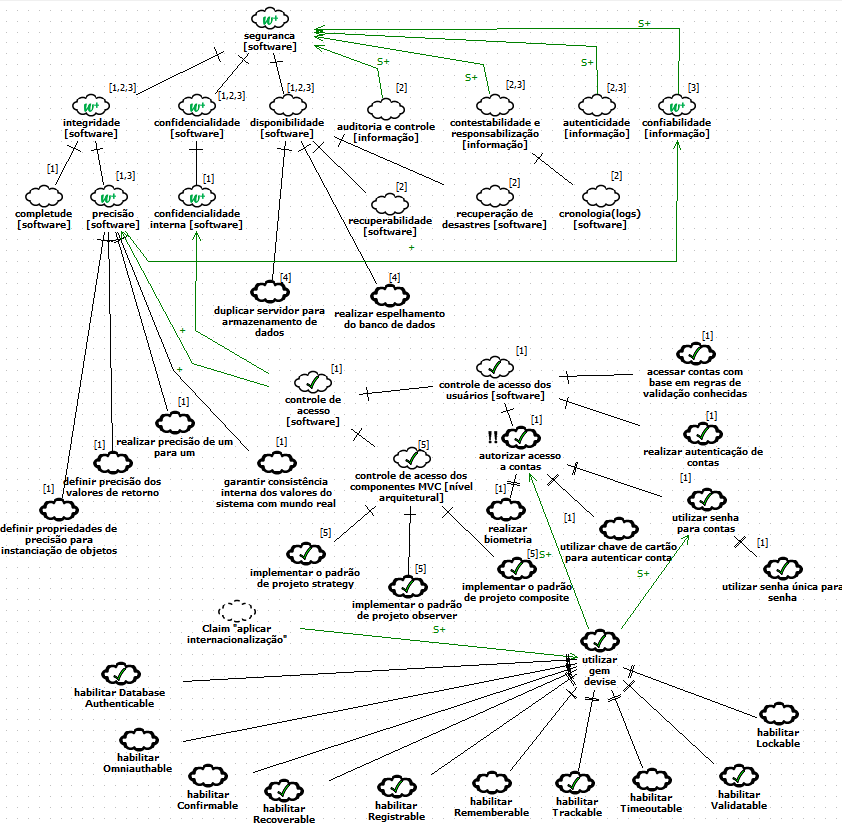
\includegraphics[keepaspectratio=true,scale=0.7]{figuras/catalogoPersona1.PNG}
	\caption{Operacionalizações para autenticação de usuário utilizando a \textit{gem devise}.}
	\label{catalogoPersona1}
\end{figure}


O Catálogo de Segurança aplicado no cenário 1 é apresentado na Figura \ref{catalogoPersona1}, na qual as operacionalizações foram incrementadas ao catálogo inicial. Respeitando os módulos da \textit{gem devise}, a operacionalização  “autorizar acesso a contas” passou a possuir alto grau de prioridade devido ao cenário, pois esta é uma das operacionalizações que impactam diretamente a solução para o problema. 

É possível, então, utilizando a notação do NFR \textit{Framework}, realizar a modelagem da \textit{gem devise} como uma operacionalização, representando a existência de alguma contribuição positiva (SOME+) com as operacionalizações  “autorizar acesso a contar” e “utilizar senha para contas”.
 
As operacionalizações filhas de “utilizar \textit{gem devise}” e que atendem as necessidades da persona descrita no cenário 1 são:

\begin{itemize}
	\item “habilitar \textit{Database Authenticatable}”: é um dos requisitos mínimos para que ocorra a persistência da senha no banco de dados;
	\item “habilitar \textit{Recoverable}”: capacidade de redefinir a senha do usuário;
	\item “habilitar \textit{Registrable}”: é um dos requisitos mínimos e que permite a inscrição de usuários; 
	\item “habilitar \textit{Trackable}”: monitorar a quantidade de entradas do usuário, e 
	\item “habilitar \textit{Validatable}”: validar conta via email do usuário. 
\end{itemize}

Portanto, ao habilitar os módulos da \textit{gem devise} dentro da camada \textit{model}, nas classes \textit{Admins} e \textit{Members}, as operacionalizações são satisfeitas. Podemos então, verificar qual nível de satisfação da segurança do software pode ser alcançado com a utilização da \textit{gem devise}. 

O trecho de código abaixo apresenta como pode ser os módulos podem ser habilitados.  
 
\begin{lstlisting} 
class Admins < ApplicationRecord
devise :database_authenticatable, :registerable,
:recoverable, :rememberable, :trackable, :validatable
end 
\end{lstlisting} 

A implementação dos padrões de projeto \textit{strategy}, \textit{observer} e \textit{composite} já estão suficientemente satisfeitos, pois a aplicação é desenvolvida com o \textit{framework rails} que obedece o padrão MVC e a \textit{gem} que está sendo utilizada também percorre todas as camadas. 

\section{Cenário 2}
\label{subsec:persona2}

Pedro, 23 anos, Engenheiro de Software, trabalha em empresa privada e possui a necessidade de desenvolver o sistema da ouvidoria da instituição. Tal sistema deverá ser desenvolvido em plataforma web para atender os processos de manifestação (denúncia, reclamação, solicitação, sugestão e elogio) realizados pela ouvidoria. Esse tipo de informação deve ser estritamente confidencial, podendo ou não, o manifestante ser anônimo.  

\begin{itemize}
	\item O problema: sobrecarga de manifestações sem interação com os manifestantes; 
	\item Objetivo: promover a interação anônima ou forma entre a ouvidora e o manifestante, e
	\item Desafio: realizar a interação anônima entre ouvidora e manifestante, que permita a execução dos processos de auditória e controle das manifestações.
\end{itemize}

\subsection{Identificar possível solução}

Uma possível solução é gerar um número de protocolo, durante o registro da manifestação, para que possa ser realizado o acompanhamento. Tal número será utilizado tanto para a manifestação anônima, quanto para a manifestação formal. O manifestante poderá acompanhar o status de sua manifestação através da visão de acompanhamento, na qual ficarão registradas as respostas dadas pela ouvidora.

A Ouvidora, no caso, acessará o sistema de forma diferente, utilizando a área administrativa do sistema através da autenticação de usuário. Ao fazer isso, a mesma estará apta a visualizar todas as manifestações e selecionar a desejada, para que seja possível a redação da resposta para o manifestante.  

\subsection{Aplicação do Catálogo de Segurança}

\begin{figure}[h!]
	\centering
	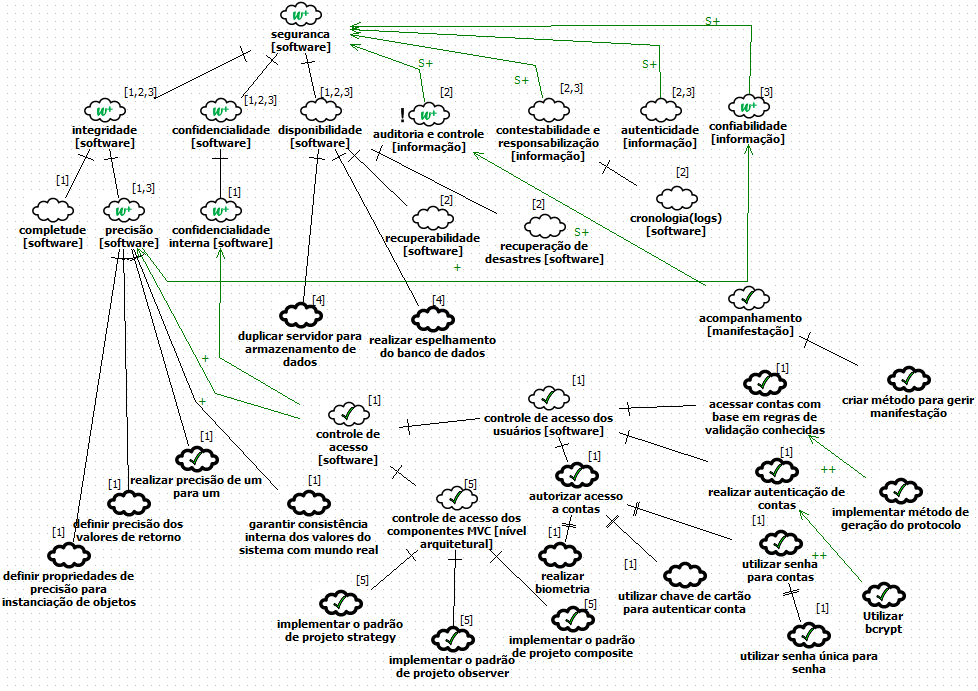
\includegraphics[keepaspectratio=true,scale=0.6]{figuras/catalogoPersona2.PNG}
	\caption{Catálogo de segurança aplicado ao sistema de ouvidoria.}
	\label{catalogoPersona2}
\end{figure}



Na aplicação do Catálogo de Segurança da figura \ref{catalogoPersona2}, surgiu a necessidade de focar em  “auditoria e controle”, pois o cenário demandava  o acompanhamento das manifestações pelos ouvidores. Com isso, foi expandido no Catálogo de Segurança uma nova meta flexível “Realizar acompanhamento das manifestações” e uma operacionalização “Criar método para gerir manifestação”. A operacionalização é definida pelos métodos implementados na \textit{controller - ManagerManifestationsController}. Portanto, a meta flexível “auditoria e controle” é suficientemente satisfeita para este contexto.

Para que a meta flexível “controle de acesso dos usuários” seja suficientemente satisfeita, as três operacionalizações que estão no nível mais baixo no Catálogo de Segurança também serão, sendo elas: (i) “implementar método de geração do protocolo”: trata-se de um método para gerar os números de protocolos com caracteres (de “a” à “z”), (de “A” à “Z”) e (de “0” à “9”) composto por 10 dígitos; (ii) “utilizar senha única para senha”: para cada usuário administrador/ouvidor cadastrado no sistema é gerada uma única senha para autenticação; e (iii) “utilizar bcrypt”: refere-se a uma \textit{gem} que utiliza algoritmo de \textit{hashing} criptográfico trata um trecho do dado para gerar um \textit{hash}. Considerando que, ao gerar uma senha dessa maneira, trata-se da execução de um processo não reversível, visto que não há como retornar da \textit{hash} para a senha \cite{brcypt}.

A operacionalização “realizar precisão de um para um” é suficientemente satisfeita, pois para cada manifestação ocasionada por determinado evento de manifestação do mundo real existirá uma única manifestação no sistema.

Diante do exposto, observa-se que a segurança do software é parcialmente satisfeita devido a satisfação parcial da integridade e da confidencialidade do mesmo.

\section{Cenário 3}
\label{subsec:persona3}

Milena, 22 anos, Engenheira de Software, possuindo várias atividades no seu dia-a-dia, sentiu a necessidade de organizá-las e para isso, considerando as suas habilidades, decidiu escrever um programa com o objetivo de obter melhor controle sobre as mesmas. Esse programa permite a inserção da atividade com sua descrição, a data de início, a previsão de conclusão e seu status. Consequentemente, Milena optou por fazer seu sistema em \textit{Rails} e decidiu verificar as relações entre as camadas do sistema com o foco em segurança.

\begin{itemize}
	\item O problema: desorganização das atividades diárias;
	\item Objetivo: desenvolvimento de sistema para auxiliar na organização das atividades, e
	\item Desafio: verificar as relações entre as camadas do sistema com foco em segurança.
\end{itemize}


\subsubsection{Aplicação do Catálogo de Segurança}

Na descrição da persona, houve a necessidade de vincular cada atividade do mundo real com ao menos uma entidade no sistema. Para isso utilizou-se o comando \textit{scaffold} do \textit{Rails}. Tal comando gera a estrutura de arquivos de acordo com o padrão MVC, gerando o \textit{model}, o \textit{controller}, os \textit{views} necessários \cite{railscommunity}. 

\begin{figure}[h!]
	\centering
	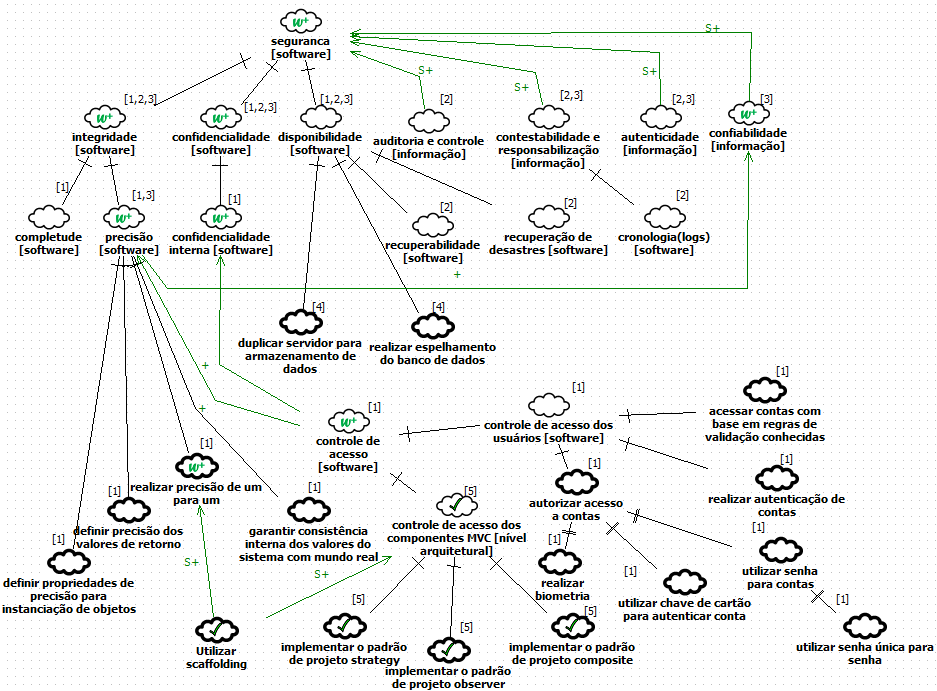
\includegraphics[keepaspectratio=true,scale=0.7]{figuras/catalogoPersona3.PNG}
	\caption{O \textit{scaffolding} do \textit{Rails} no Catálogo de Segurança.}
	\label{catalogoPersona3}
\end{figure}

Como pode ser observado na Figura \ref{catalogoPersona3}, a operacionalização “utilizar scaffolding” foi extendida ao Catálogo de Segurança, e suficientemente satisfeita devido a implementação ao cenário, satisfazendo parcialmente a operacionalização  “realizar precisão de um para um”. Portanto as outras metas flexíveis e operacionalizações foram satisfeitas de maneira semelhante aos cenários anteriores. 

\section{Cenário 4}
\label{subsec:persona4}

Gustavo, 23 anos, Engenheiro de Requisitos de empresa privada, possui a demanda de analisar os requisitos do sistema de solicitação de documentos digitais via plataforma web. Tal sistema possui arquitetura MVC e está em constante evolução. Assim sendo, seu chefe solicitou que o mesmo fizesse uma análise dos RNFs com foco na segurança do sistema, devido a emissão de documentos com assinatura digital. 

\begin{itemize}
	\item O problema: alta demanda de solicitação de documentos pelos setores; 
	\item Objetivo: promover a geração de documentos digitais via plataforma web, e
	\item Desafio: garantir a autenticidade dos documentos solicitados.
\end{itemize}

\subsection{Identificar possível solução}

A aplicação do Catálogo de Segurança pode ser uma das maneiras de demonstrar a relação entre os RNFs do sistema, principalmente, quando o RNF que está em foco é segurança.


\subsection{Aplicação do Catálogo de Segurança}

\begin{figure}[h!]
	\centering
	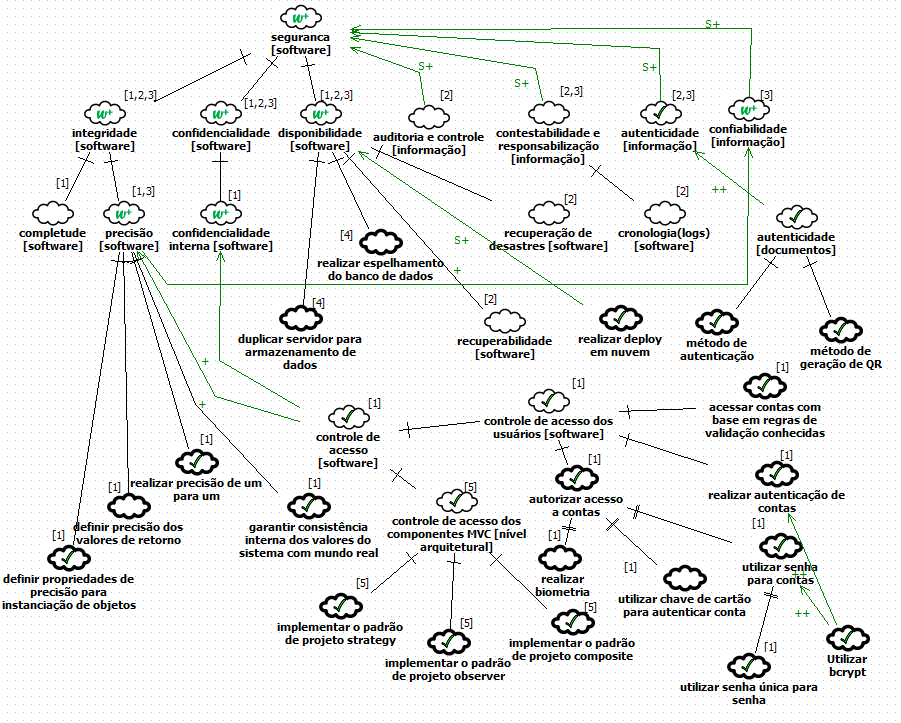
\includegraphics[keepaspectratio=true,scale=0.8]{figuras/catalogoPersona4.PNG}
	\caption{Catálogo de Segurança aplicado a sistema de geração de documentos digitais.}
	\label{catalogoPersona4}
\end{figure}

A aplicação do Catálogo de Segurança apresentado na Figura \ref{catalogoPersona4} possui uma extensão devido a utilização de assinatura digital nos documentos, que é modelada como uma meta flexível que está suficientemente satisfeita, pois depende de duas operacionalizações. As operacionalizações fazem uma relação do tipo AND com a meta flexível e ambas estão suficientemente satisfeitas, sendo elas “método de geração de (\textit{Quick Response} Quick) QR” e o  “método de autenticação” que utiliza valores como o identificador do usuário e a \textit{string} do QR. Essas relações satisfazem suficientemente a meta flexível para autenticidade da informação. 

O controle de acesso do software é satisfeito devido a relação das metas flexíveis e operacionalizações, da mesma forma que os cenários \ref{subsec:persona2} e \ref{subsec:persona1} anteriores, que já apresentaram os mesmos relacionamentos, com mesmos níveis de satisfação.  

Já a operacionalização “definir propriedades de precisão para instanciação de objetos” é escrita em cada \textit{model}, onde o \textit{Rails} permite escrever os parâmetros para controle de instanciação dos objetos. Neste cenário, foi aplicado que o atributo da classe tem que existir no banco de dados, não podendo colocar vazio ou nulo. 

A aplicação está em um servidor da Google, na nuvem, garantindo sua disponibilidade e satisfazendo então, suficientemente a operacionalização “realizar deploy em nuvem”. 

Semelhante as aplicações dos cenários \ref{subsec:persona2} e \ref{subsec:persona3} a “precisão de um para um” é suficientemente satisfeita. 

\section{Cenário 5}
\label{subsec:persona5}

Chung, 40 anos, Engenheiro de Software possui em seu quadro de responsabilidades a função de realizar manutenção e evolução de um dos sistemas pelo qual é responsável. Desse modo, percebeu que um de seus sistemas poderia ficar indisponível caso ocorresse algum problema no servidor de banco de dados. Preocupado com a segurança de seus sistemas, utilizou o Catálogo de Segurança para analisar o impacto que o espelhamento da base de dados causaria na segurança do software como um todo. 

\begin{itemize}
	\item O problema: indisponibilidade do sistema; 
	\item Objetivo: garantir a base disponível para ser utilizada pelo sistema, e
	\item Desafio: manter a base de dados disponível diante de qualquer interrupção de serviço e que possa impedir acesso ao mesmo.
\end{itemize}

\subsection{Aplicação do Catálogo de Segurança}

\begin{figure}[h!]
	\centering
	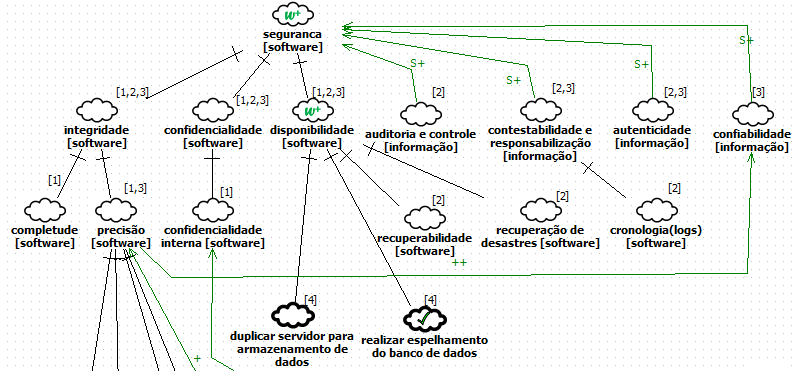
\includegraphics[keepaspectratio=true,scale=0.7]{figuras/catalogoPersona5.PNG}
	\caption{Catálogo de Segurança com foco em disponibilidade aplicado ao contexto de duplicação de base de dados.}
	\label{catalogoPersona5}
\end{figure}

A operacionalização “espelhamento da base de dados” é suficientemente satisfeita, satisfazendo parcialmente a disponibilidade do software. Esse cenário, em especial, foi modelado justamente para demonstrar o impacto de ações realizadas na base de dados na segurança do software, como apresentado na Figura \ref{catalogoPersona5}.


\section{Primeira visão do Catálogo de Segurança após as aplicações nos cenários}
\label{sec:aplicacaoDoCatalogo}

Ao modelar o Catálogo de Segurança pela primeira vez sem ter realizado nenhuma interação com algum tipo de cenário, obteve-se visão preliminar sobre Segurança devido à subjetividade e ao conjunto de conceitos abstratos presentes na literatura.  

Ao demonstrar a aplicação do Catálogo de Segurança nos cenários, observou-se que o mesmo permite, não somente a visão preliminar da segurança de software, mas também de segurança da informação.

Como o Catálogo de Segurança foi aplicado em cenários onde a ferramenta de apoio ao desenvolvimento era o \textit{Rails}, foi possível abstraí-lo para aplicações em \textit{Rails}, demonstrando então, a adaptabilidade do mesmo, como pode ser visualizado na Figura \ref{catalogoFull}.

\begin{figure}[h!]
	\centering
	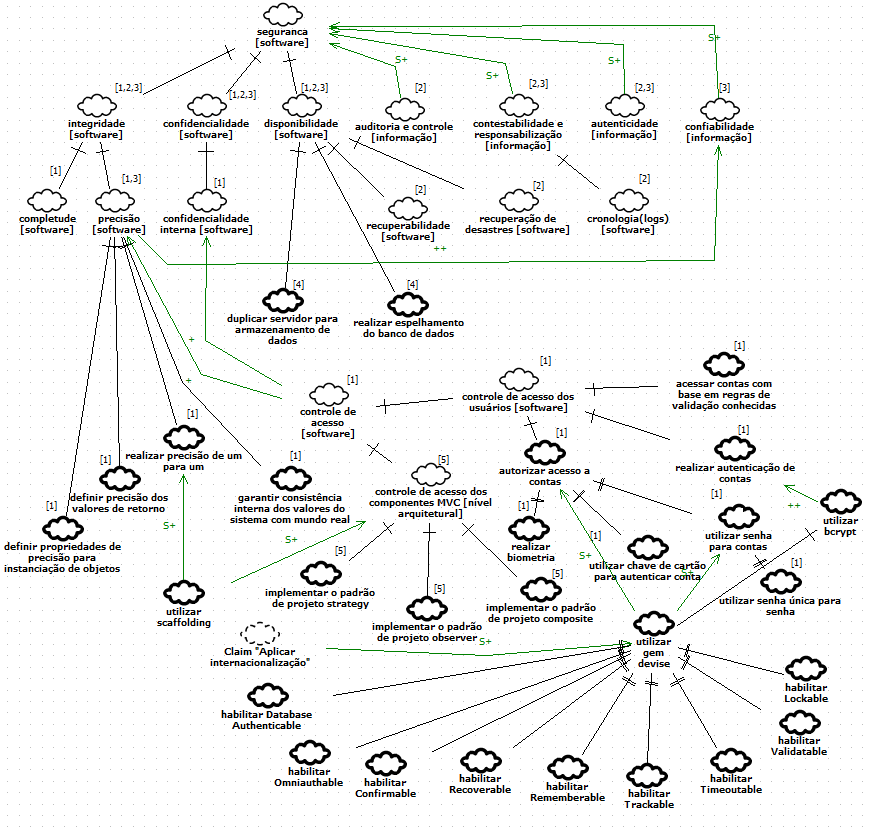
\includegraphics[keepaspectratio=true,scale=0.65]{figuras/catalogoFull.PNG}
	\caption{Versão extendida do Catálogo de Segurança focada em projetos \textit{Rails}.}
	\label{catalogoFull}
\end{figure}


Entretanto, durante a validação do Catálogo de Segurança, foram utilizados projetos em cenários reais e abstrações de possíveis usuários e cenários, tornando-o mais abrangente, caso a tecnologia utilizada seja o \textit{Rails}. Como um exemplo de evolução do Catálogo de Segurança e as evidências comprovadas da relação entre as operacionalizações e as camadas do Padrão Arquitetural MVC, é possível unificar com fins de demonstração o Catálogo de Segurança com um diagrama de componentes do padrão MVC, onde as operacionalizações estão dentro do componente ao qual possui relacionamento, como pode ser visualizado na Figura \ref{catalogoMapeado}. 


\begin{comment}
	A Tabela \ref{resultadosObtidos} apresenta de acordo com os objetivos específicos do trabalho, usando "atendido", "parcialmente atendido" e "não atendido", os principais resultados obtidos até o momento, com a realização do TCC1.	
\end{comment}

\begin{figure}[h!]
	\centering
	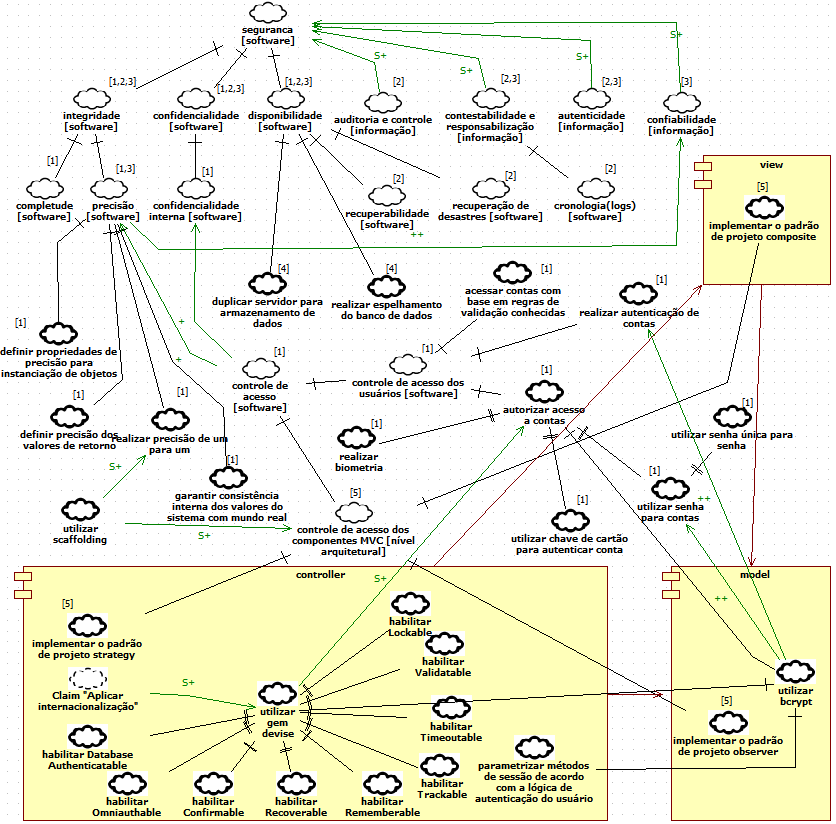
\includegraphics[keepaspectratio=true,scale=0.7]{figuras/catalogoMapeado.PNG}
	\caption{Mapeamento das metas flexíveis e operacionalizações com as camadas do MVC.}
	\label{catalogoMapeado}
\end{figure}

\pagebreak

\section*{Resumo do Capítulo}

Neste capítulo, foram apresentadas as primeiras aplicações do Catálogo de Segurança, realizadas através de cinco cenários, onde foi possível demonstrar a aplicabilidade e a adaptabilidade do Catálogo de Segurança, de acordo com o contexto. A partir da seção \ref{sec:aplicacaoDoCatalogo}, foi possível evidenciar a evolução do Catálogo de Segurança para as aplicações em projetos em \textit{Rails} e, por fim, o mapeamento em terceiro nível de abstração, sendo possível identificar as operacionalizações relacionadas com as camadas do Padrão Arquitetural MVC para projetos em \textit{Rails}.


